% begin module max-min-def
\begin{frame}[t]
\begin{columns}[c]
\column{.5\textwidth}

\psset{xunit=0.8cm, yunit=0.8cm}
\begin{pspicture}(-5, -5)(5,5) 
\psframe*[linecolor=white](-5,-5)(5,5) 
\psaxes[ticks=none, labels=none]{<->}(0,0)(-0.5,-0.5)(5,4.5)
%Function formula: 657/250+2/3 ((-1/2+x)^{2}) 
\psplot[linecolor=red, plotpoints=1000]{0}{1.2}{x -0.5 add 2 exp 0.666667 mul 2.628 add } %Function formula: -6 (x)-2/3 ((-1+x)^{3})+10+4 ((-1+x)^{2}) 
\psplot[linecolor=red, plotpoints=1000]{1.2}{4.5}{x -1 add 2 exp 4 mul 10 add x -1 add 3 exp -0.666667 mul add x -6 mul add }
\tiny
\only<handout:0|12,13,14>{%
\psFullDot{0.5}{2.628}
\psline[linestyle=dashed](0.5, 2.628)(0.5,0)
}
\psline(0.5,-0.1)(0.5,0.1)
\rput[t](0.5,-0.15){$a$}

\only<handout:0|8,9,10>{%
\psFullDot{1.2}{2.95467}
\psline[linestyle=dashed](1.2, 2.95467)(1.2,0)
}
\psline(1.2,-0.1)(1.2,0.1)
\rput[t](1.2,-0.15){$b$}

\only<handout:0 | 10>{ %
\psFullDot{0}{2.79467}
}

\only<handout:0| 5,13,14>{%
\psFullDot{2}{1.33333}
\psline[linestyle=dashed](2,1.33333)(2,0)
}
\psline(2,-0.1)(2,0.1)
\rput[t](2,-0.15){$c$}

\only<handout:0| 3, 9,10>{%
\psFullDot{4}{4}
\psline[linestyle=dashed](4,4)(4,0)
}
\psline(4,-0.1)(4,0.1)
\rput[t](4,-0.15){$d$}

\only<handout:0| 14>{%
\psFullDot{4.5}{3.41667}
\psline[linestyle=dashed](4.5,3.41667)(4.5,0)
}
\psline(4.5,-0.1)(4.5,0.1)
\rput[t](4.5,-0.15){$e$}
\end{pspicture} 
%\ \only<-2,4,6-7,10>{%
%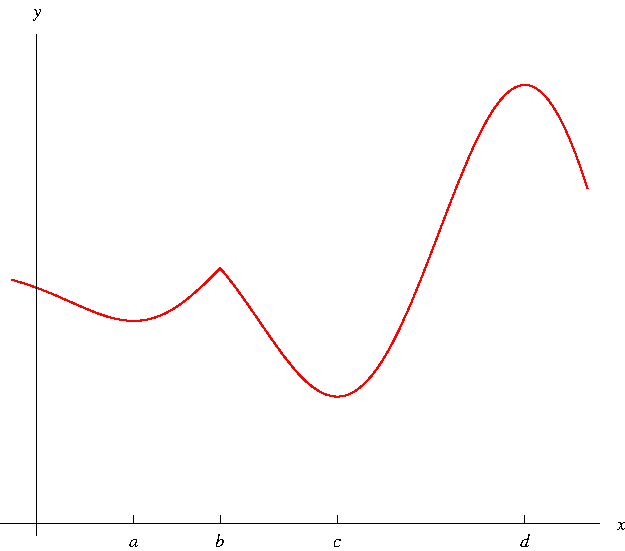
\includegraphics[width=5.5cm]{maxima-minima/pictures/04-01-minmaxa.pdf}%
%}%
%\only<handout:0| 3,9>{%
%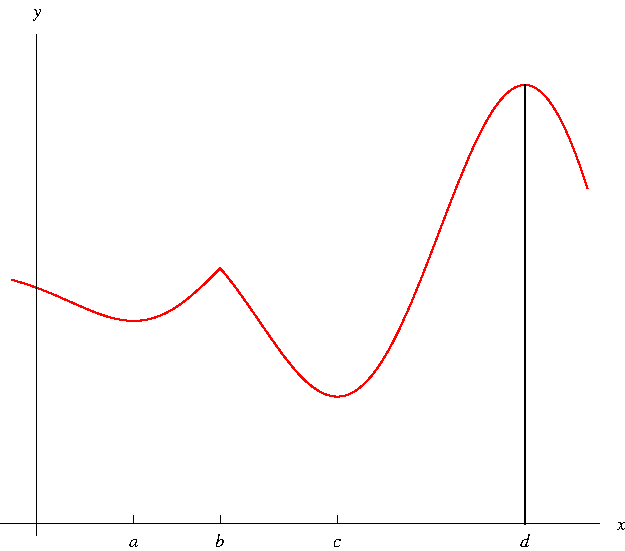
\includegraphics[width=5.5cm]{maxima-minima/pictures/04-01-minmaxe.pdf}%
%}%
%\only<handout:0| 5,12>{%
%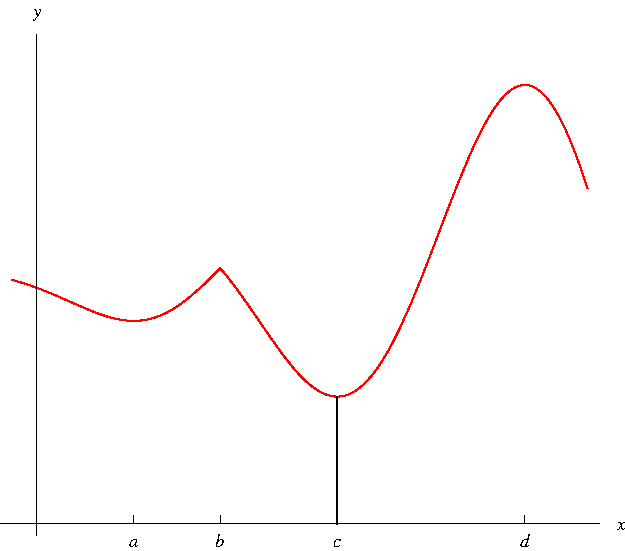
\includegraphics[width=5.5cm]{maxima-minima/pictures/04-01-minmaxd.pdf}%
%}%
%\only<handout:0| 8>{%
%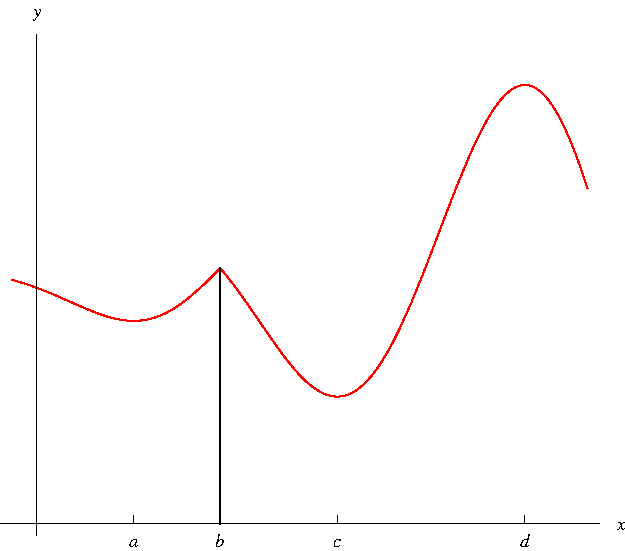
\includegraphics[width=5.5cm]{maxima-minima/pictures/04-01-minmaxc.pdf}%
%}%
%\only<handout:0| 11>{%
%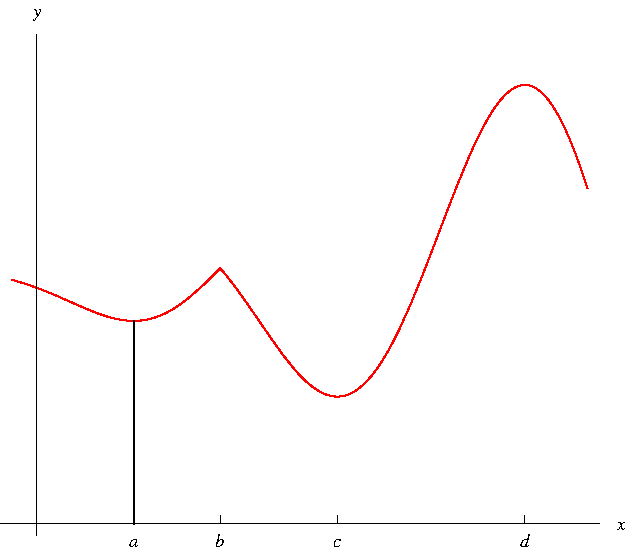
\includegraphics[width=5.5cm]{maxima-minima/pictures/04-01-minmaxb.pdf}%
%}%

\column{.5\textwidth}
\begin{itemize}
\item<2-| alert@2-3>  Absolute maximum at \uncover<3->{$d$}.
\item<2-| alert@4-5>  Absolute minimum at \uncover<5->{$c$}.
\item<7-| handout:2| alert@7-9>  Local maximum at \uncover<8->{$b$,} \uncover<9->{$d$} \uncover<10->{and $0$.}
\item<7-| handout:2| alert@11-12>  Local minimum at \uncover<12->{$a$,} \uncover<13->{ $c$ and }  \uncover<14->{$e$.}
\end{itemize}
\end{columns}
\only<handout:1| -5>{%
\begin{definition}[Absolute Maximum or Minimum]
A function $f$ has an absolute maximum (or global maximum) at $c$ if $f(c) \geq f(x)$ for all $x$ in the domain of $f$.  The number $f(c)$ is called the maximum value of $f$.

Likewise, $f$ has an absolute minimum at $c$ if $f(c) \leq f(x)$ for all $x$ in the domain of $f$.  $f(c)$ is called the minimum value of $f$.

Maximum and minimum values of $f$ are called extreme values.
\end{definition}
}%
\only<handout:2| 6->{%
\begin{definition}[Local Maximum or Minimum]
A function $f$ has a local maximum at $c$ if $f(c) \geq f(x)$ for all $x$ in some open interval containing $c$.  Similarly, $f$ has a local minimum at $c$ if $f(c) \leq f(x)$ for all $x$ in some open interval containing $c$.
\end{definition}
}%
\end{frame}
% end module max-min-def
